% --------------------------------------------------------------------------------
\newpage
\section{Onset Module}
% --------------------------------------------------------------------------------

% Make general target
\hypertarget{Concepts:OnsetModule}{}

% Make target for following functions:
\hypertarget{Concepts:IPEMCalcOnsets}{}
\hypertarget{Concepts:IPEMCalcOnsetsFromANI}{}
\hypertarget{Concepts:IPEMDoOnsets}{}
\hypertarget{Concepts:IPEMOnsetPattern}{}
\hypertarget{Concepts:IPEMOnsetPatternFilter}{}
\hypertarget{Concepts:IPEMOnsetPeakDetection}{}
\hypertarget{Concepts:IPEMOnsetPeakDetection1Channel}{}
\hypertarget{Concepts:IPEMSnipSoundFileAtOnsets}{}

\subsection{Introductory description}
% --------------------------------------------------------------------------------
The onset module (OM) finds the onsets of sound events. The module
takes sound as input and produces the moments where a new note,
chord or sound event is triggered in the musical signal. Its place
in the image transformation chart is shown in figure
\ref{Fig:ModulesOM}.
\begin{figure}[h]
    \centering
    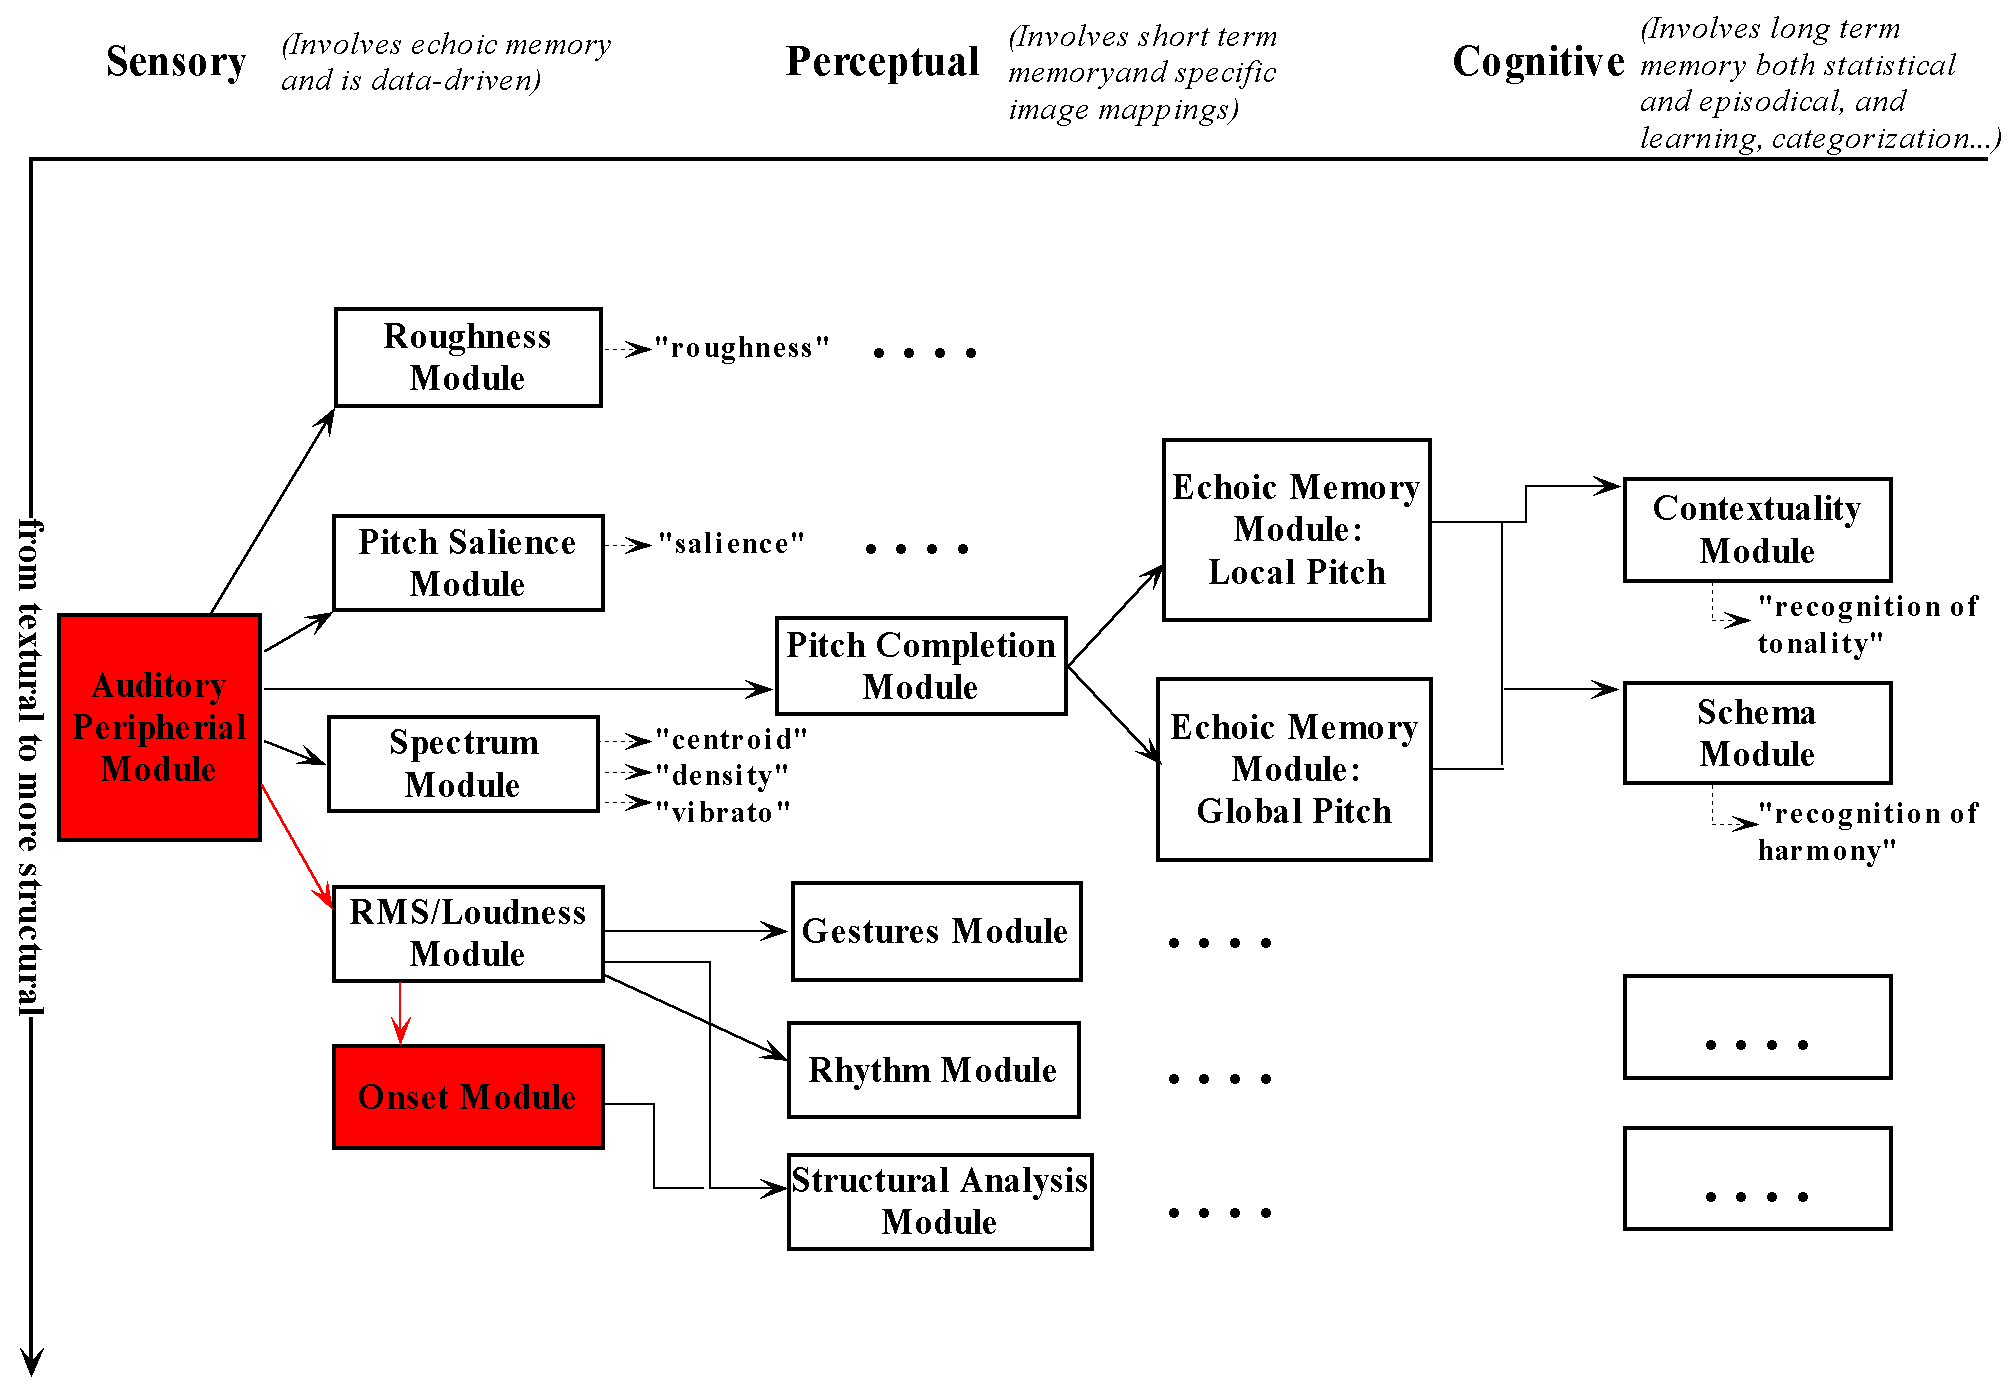
\includegraphics[width=\textwidth]{Graphics/ModulesOM}
    \caption{Chart of image transformation modules, with OM highlighted}
    \label{Fig:ModulesOM}
\end{figure}

The onset module analyzes the energy in the different auditory
channels. It extracts the relevant peaks and combines the results
for each channel to an overall onset estimation. Keep in mind that
onset detection is a rather difficult enterprise due to the fact
that some music instruments (violin, human voice, ...) have
gliding onsets which are hard to detect. Our onset module can be
used to chunk the frame-based representation into an event-based
representation. Figure \ref{Fig:OMModule} shows the modules
involved in the transformation process.
\begin{figure}[h]
    \centering
    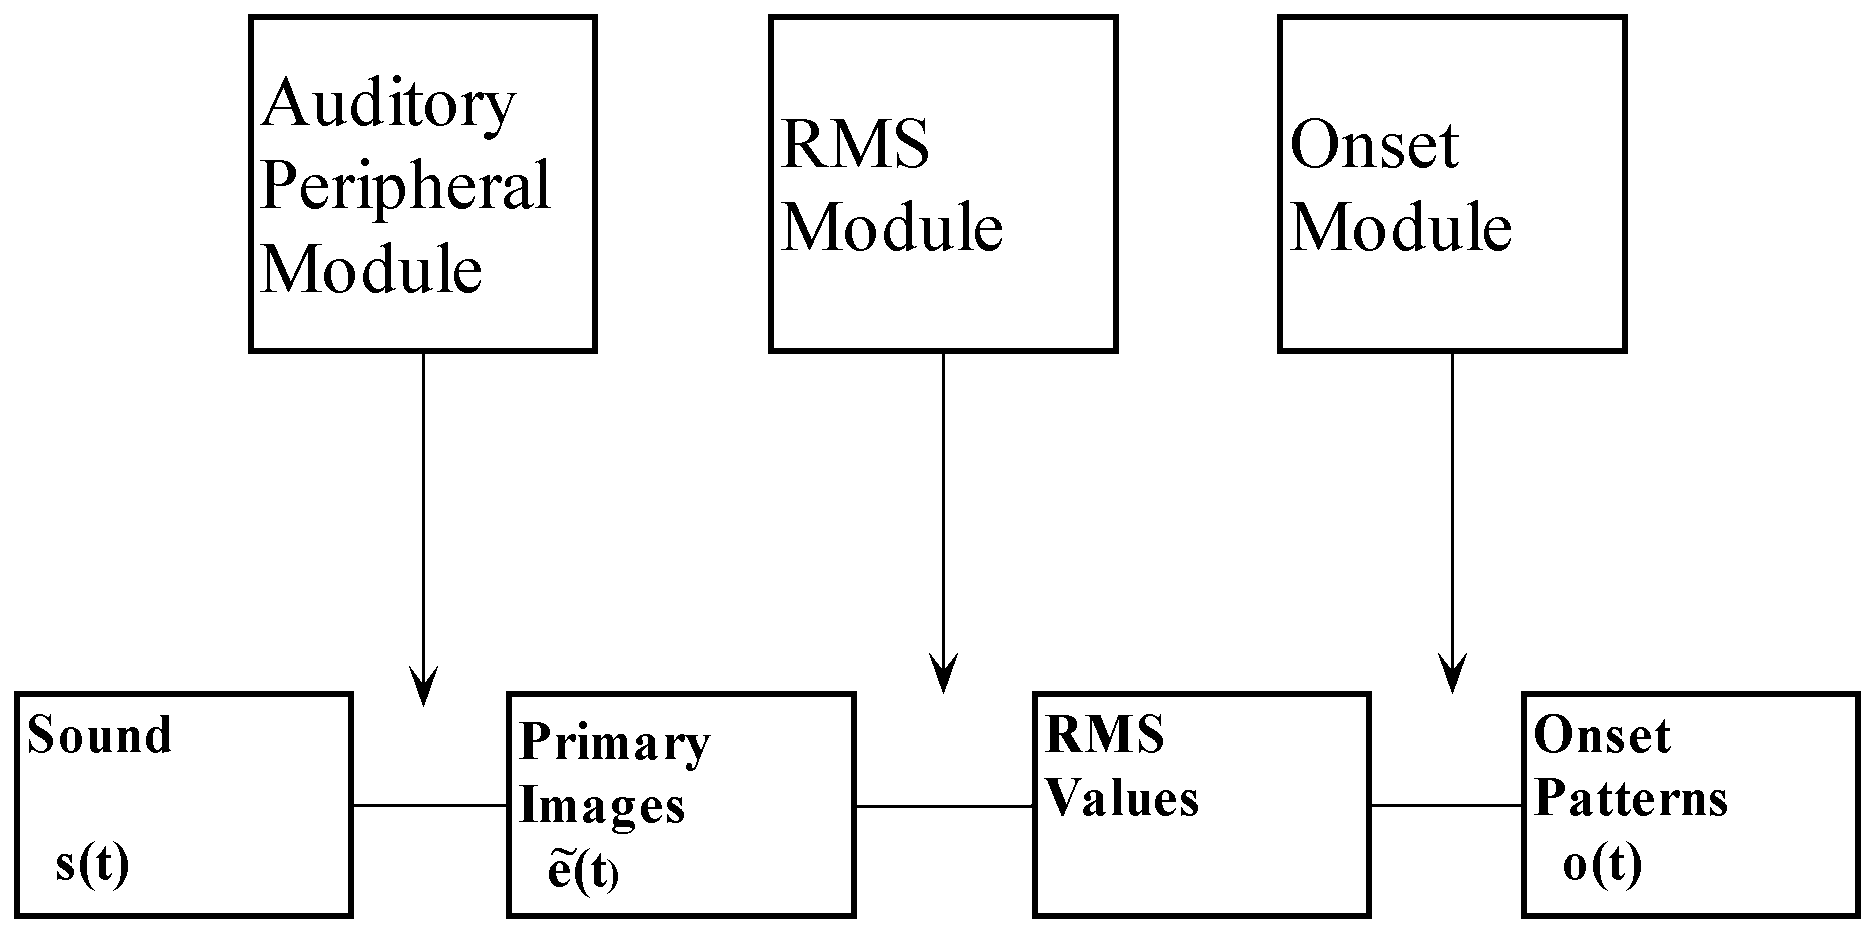
\includegraphics[width=\IPEMDefaultFigureWidth]{Graphics/OMModule}
    \caption{Modules involved for onset estimation.}
    \label{Fig:OMModule}
\end{figure}

\subsection{Functional-logical description}
% --------------------------------------------------------------------------------

The onset module involves:
\[APM: s(t) \rightarrow \tilde{e}(t)\]
\[RMS: \tilde{e}(t) \rightarrow \widetilde{rms}(t)\]
\[OM: \widetilde{rms}(t) \rightarrow o(t)\]
where APM provides the auditory nerve images and OM transforms
these images into the signal $o(t)$. A non-zero value in $o(t)$
corresponds to an onset at that moment, the value itself being
proportional to the estimated relevance of the onset.

\subsection{Signal processing description}
% --------------------------------------------------------------------------------

The algorithm used for detection of onsets consists of the
following steps:
\begin{enumerate}
\item Calculation of auditory nerve image.\\
    The auditory nerve image is calculated
    using the \hyperlink{Concepts:AuditoryPeripheralModule}{Auditory Peripheral Module}.
\item Calculation of RMS.\\
    For each of the channels in the ANI, the root mean square values are calculated using
    a frame size of 0.029 s and a frame step of 0.0058 s.
    For each frame $F$ in each channel, an RMS value is calculated according to:
    \begin{displaymath}
    RMS = \sqrt{\frac{\displaystyle \sum_{i=1}^{N}{F_{i}^2}}{N}}
    \end{displaymath}
    where $N$ = frame width in samples, and $F_{i}$ is the i-th sample of frame
    $F$.
    There is a toolbox function for the calculation of RMS values,
    see \hyperlink{FuncRef:IPEMCalcRMS}{IPEMCalcRMS}.
\item Low pass filtering.\\
    Each of these RMS-averaged channels is filtered with a second-order low pass Butterworth filter
    with a cutoff frequency of 15 Hz. This is done to reduce small, irrelevant peaks in the RMS signal.
\item Peak detection.\\
    Detection of relevant peaks in each channel is the tricky
    part....
    We start with all true peaks: moments where the first derivative goes from positive to negative.
    Then, the following approach is used for deciding whether a peak in a channel should be kept as an
    onset candidate for that channel:
    \begin{itemize}
    \item ignore everything below a certain threshold
    \item only keep peaks that are significantly bigger than their neighbors
    \item apply a mask so that following peaks due to irrelevant vibrations are thrown out
    \item for all remaining peaks, keep the biggest ones within a certain neighborhood, but only
          if it's big enough compared to the median value at that point
    \end{itemize}
\item Application of integrate-and-fire neural network.\\
    The contribution of this part is to cluster the peaks detected in the previous step over
    all channels and over time.
    This algorithm is based on an article by \citeA{Smith:1996}.
    One integrate-and-fire neuron is used per channel.
    Each neuron receives input from a set of
    adjacent channels, accumulates its input over time
    and its output is fed back to a number
    of adjacent neurons.
    The neuron dynamics are given by:
    \begin{displaymath}
    \frac{dA}{dt} = I(t) - diss\times{A} \qquad \textrm{with:
        \begin{tabular}[t]{l}
            $A$ = neurons' accumulated value \\
            $I$ = input \\
            $diss$ = dissipation factor
        \end{tabular}
        }
    \end{displaymath}

    If a neurons' accumulated value exceeds a certain threshold, it fires and the accumulated value
    is reset to zero. After firing, the neuron becomes insensitive to input for some period,
    called the refractory period. This configuration produces a sharp bursts of spikes when a
    number of channels provide evidence for onsets.
\item Final filtering.\\
    The onset pattern is finally filtered using the following approach:
    an onset is detected at a certain moment\\
    \begin{tabular}[t]{l}
        - if a certain number of channels detected an onset within
        a specific period of time, and\\
        - if the moment falls at least a minimum period of time
        behind the last detected onset\\
    \end{tabular}
\end{enumerate}

The result of these steps is a signal where a non-zero value
indicates the presence of an onset. To get an indication for the
relevance of a specific onset, we have used the number of
channels that detected an onset divided by the total number of
channels.

\subsection{Implementation}
% --------------------------------------------------------------------------------

\begin{tabularx}{\linewidth}{llX}
\hyperlink{FuncRef:IPEMCalcOnsets}{IPEMCalcOnsets} & - & Calculates onsets of sound signal\\
\hyperlink{FuncRef:IPEMCalcOnsetsFromANI}{IPEMCalcOnsetsFromANI} & - & Calculates onsets starting from an ANI\\
\hyperlink{FuncRef:IPEMDoOnsets}{IPEMDoOnsets} & - & Calculates onsets of sound file\\
\hyperlink{FuncRef:IPEMOnsetPattern}{IPEMOnsetPattern} & - & Integrate-and-fire neural net for onset detection\\
\hyperlink{FuncRef:IPEMOnsetPatternFilter}{IPEMOnsetPatternFilter} & - & Filters onset detection peak pattern\\
\hyperlink{FuncRef:IPEMOnsetPeakDetection}{IPEMOnsetPeakDetection} & - & Detects possible onset peaks in multi-channel signal\\
\hyperlink{FuncRef:IPEMOnsetPeakDetection1Channel}{IPEMOnsetPeakDetection1Channel} & - & Detects possible onset peaks in single channel\\
\hyperlink{FuncRef:IPEMSnipSoundFileAtOnsets}{IPEMSnipSoundFileAtOnsets} & - & Cuts sound file in segments at onsets\\
\end{tabularx}


\subsection{Examples}
% --------------------------------------------------------------------------------

To extract the onsets from
\IPEMSound{Sounds/SchumannKurioseGeschichte.wav}{Schumann's
Kuriose Geschichte}, use the following expression:\\

\begin{IPEMCodeEnvironment}
[Ts,Tsmp] = IPEMDoOnsets('SchumannKurioseGeschichte.wav');
\end{IPEMCodeEnvironment}\\

You can of course split the module in the several subparts. For
example, if you first process the file with the Auditory
Peripheral Module, and then apply the onsets module, you could
use:\\

\begin{IPEMCodeEnvironment}
[ANI,ANIFreq,ANIFilterFreqs] = IPEMCalcANIFromFile('SchumannKurioseGeschichte.wav');
\newline [OnsetSignal,OnsetFreq] = IPEMCalcOnsetsFromANI(ANI,ANIFreq);
\end{IPEMCodeEnvironment}\\

Figures \ref{Fig:OnsetsANIAndRMS} to \ref{Fig:OnsetsSegmentation}
illustrate the different steps for this particular example.

\begin{figure}[h]
    \centering
    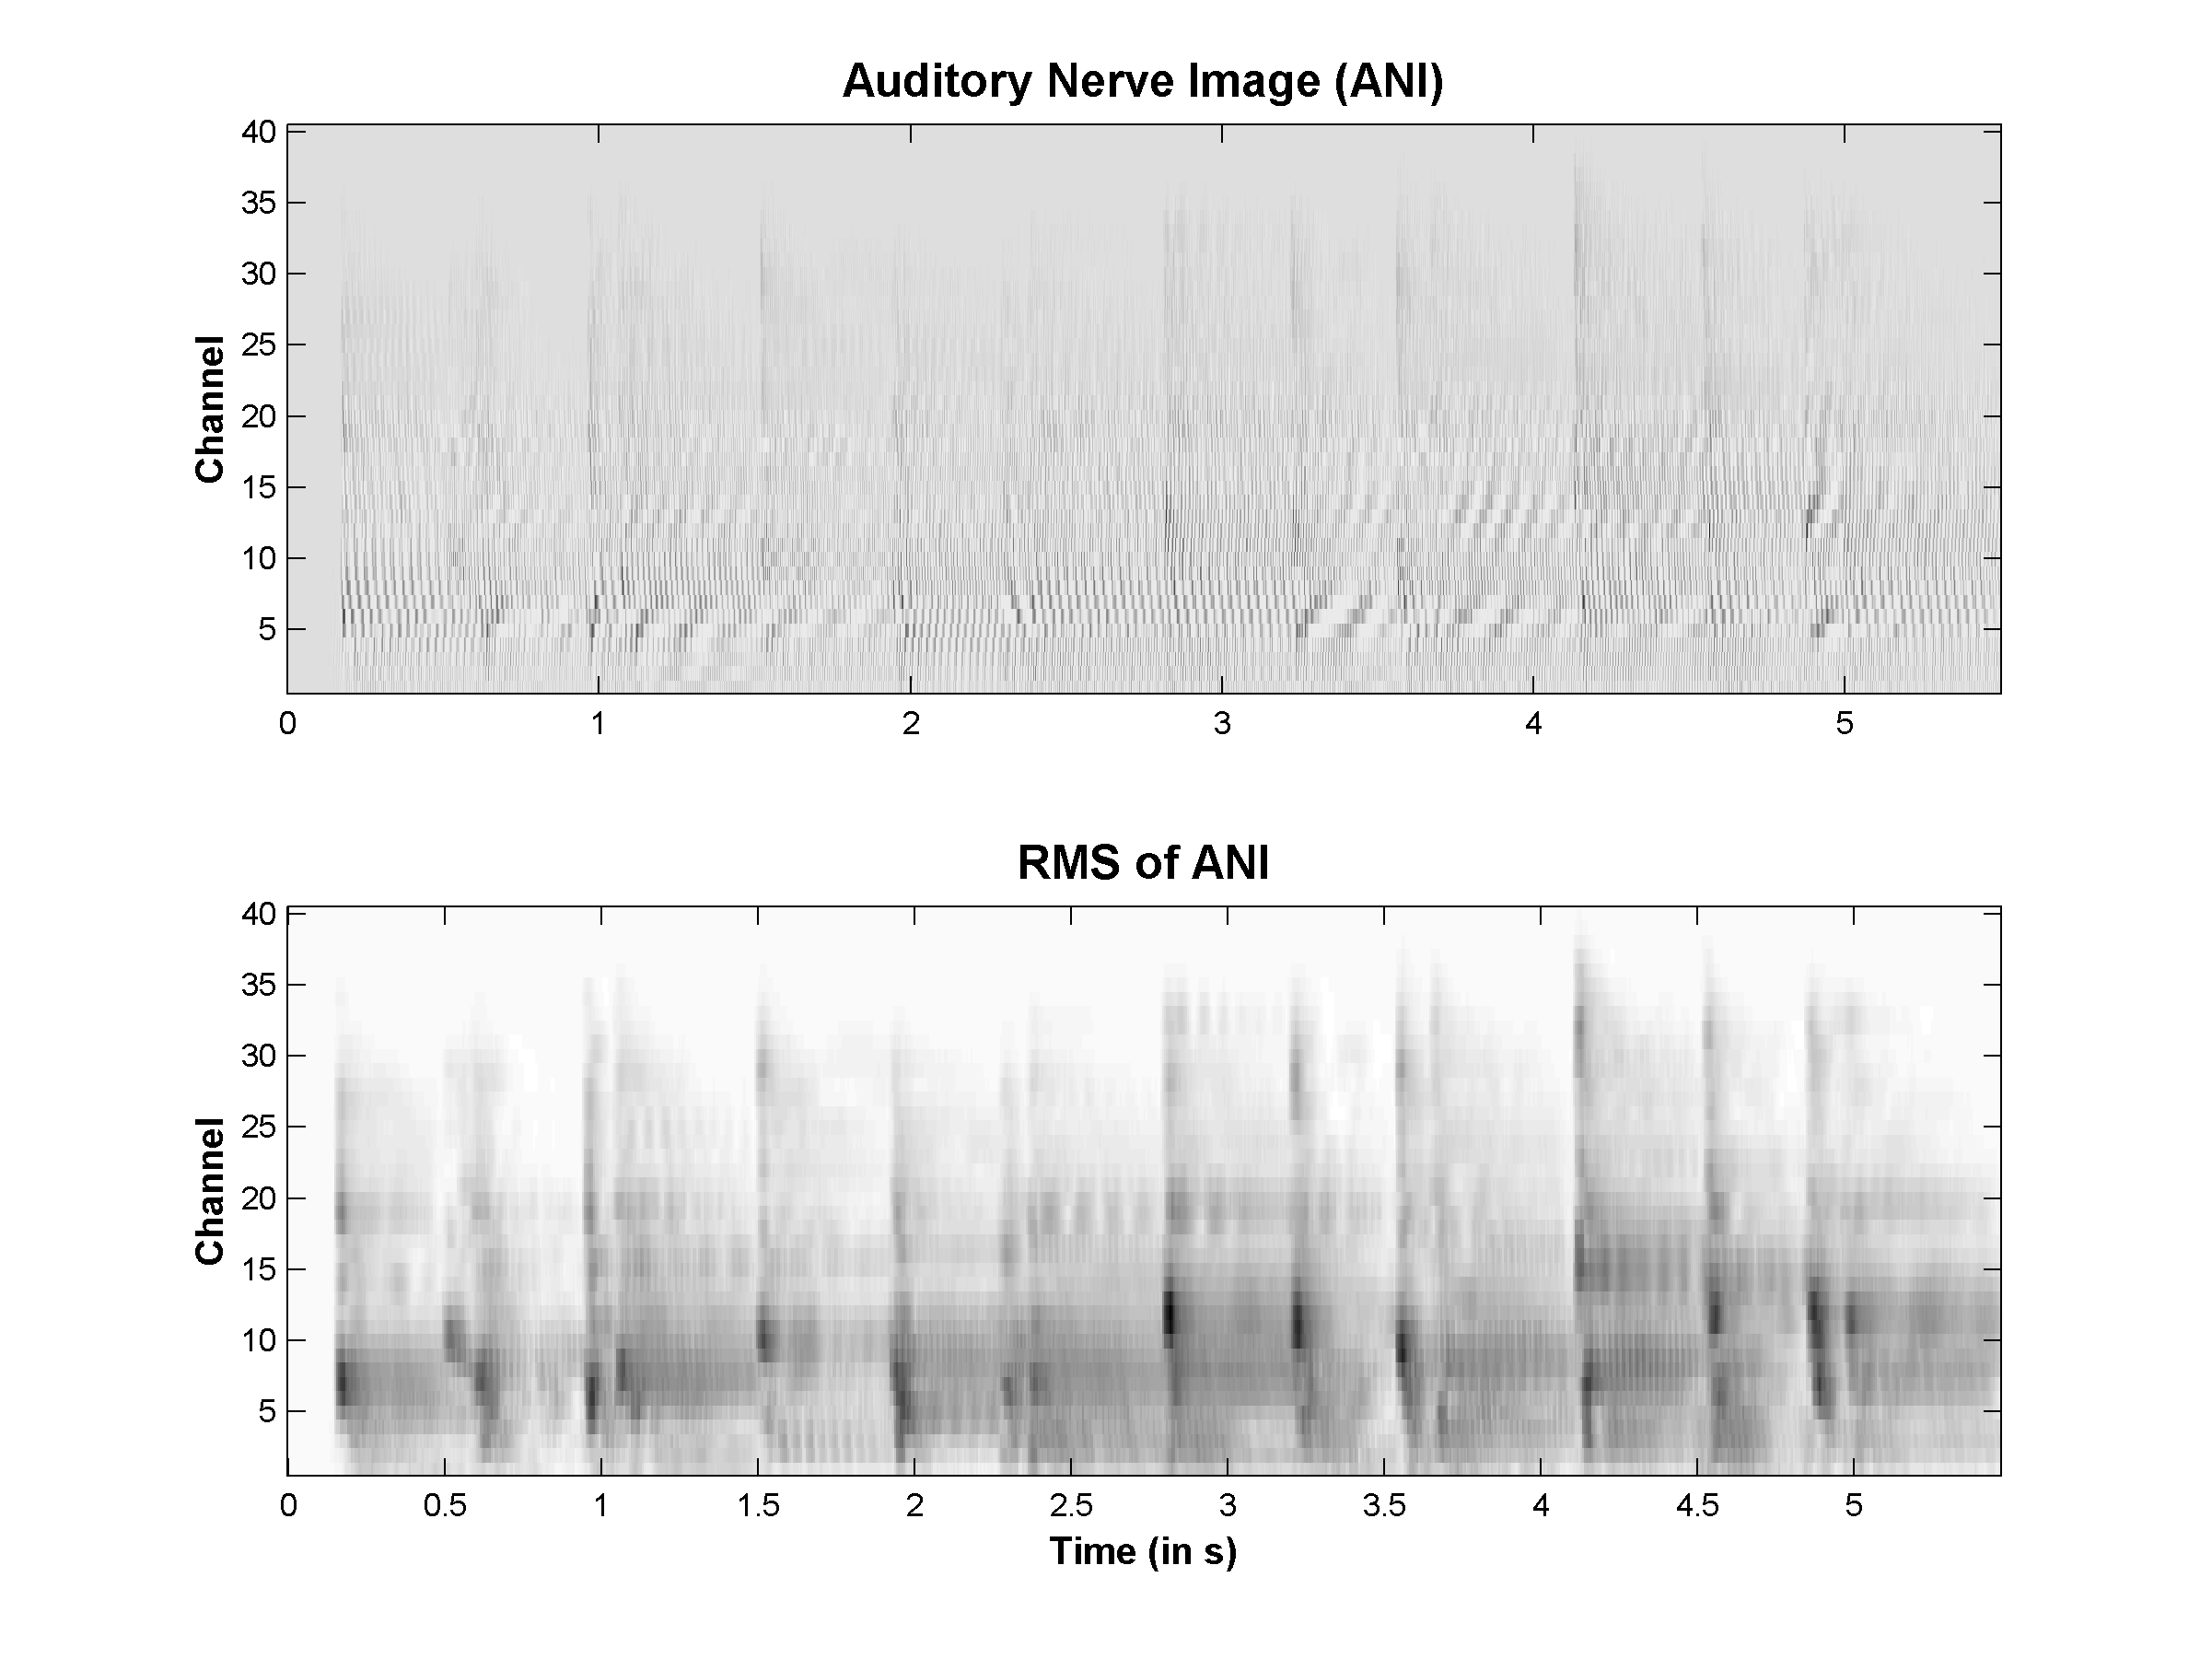
\includegraphics[width=\IPEMDefaultFigureWidth]{Graphics/OnsetsANIAndRMS}
    \caption{Top: ANI of the Schumann sound excerpt. Bottom: RMS values of the ANI.}
    \label{Fig:OnsetsANIAndRMS}
\end{figure}

\begin{figure}[h]
    \centering
    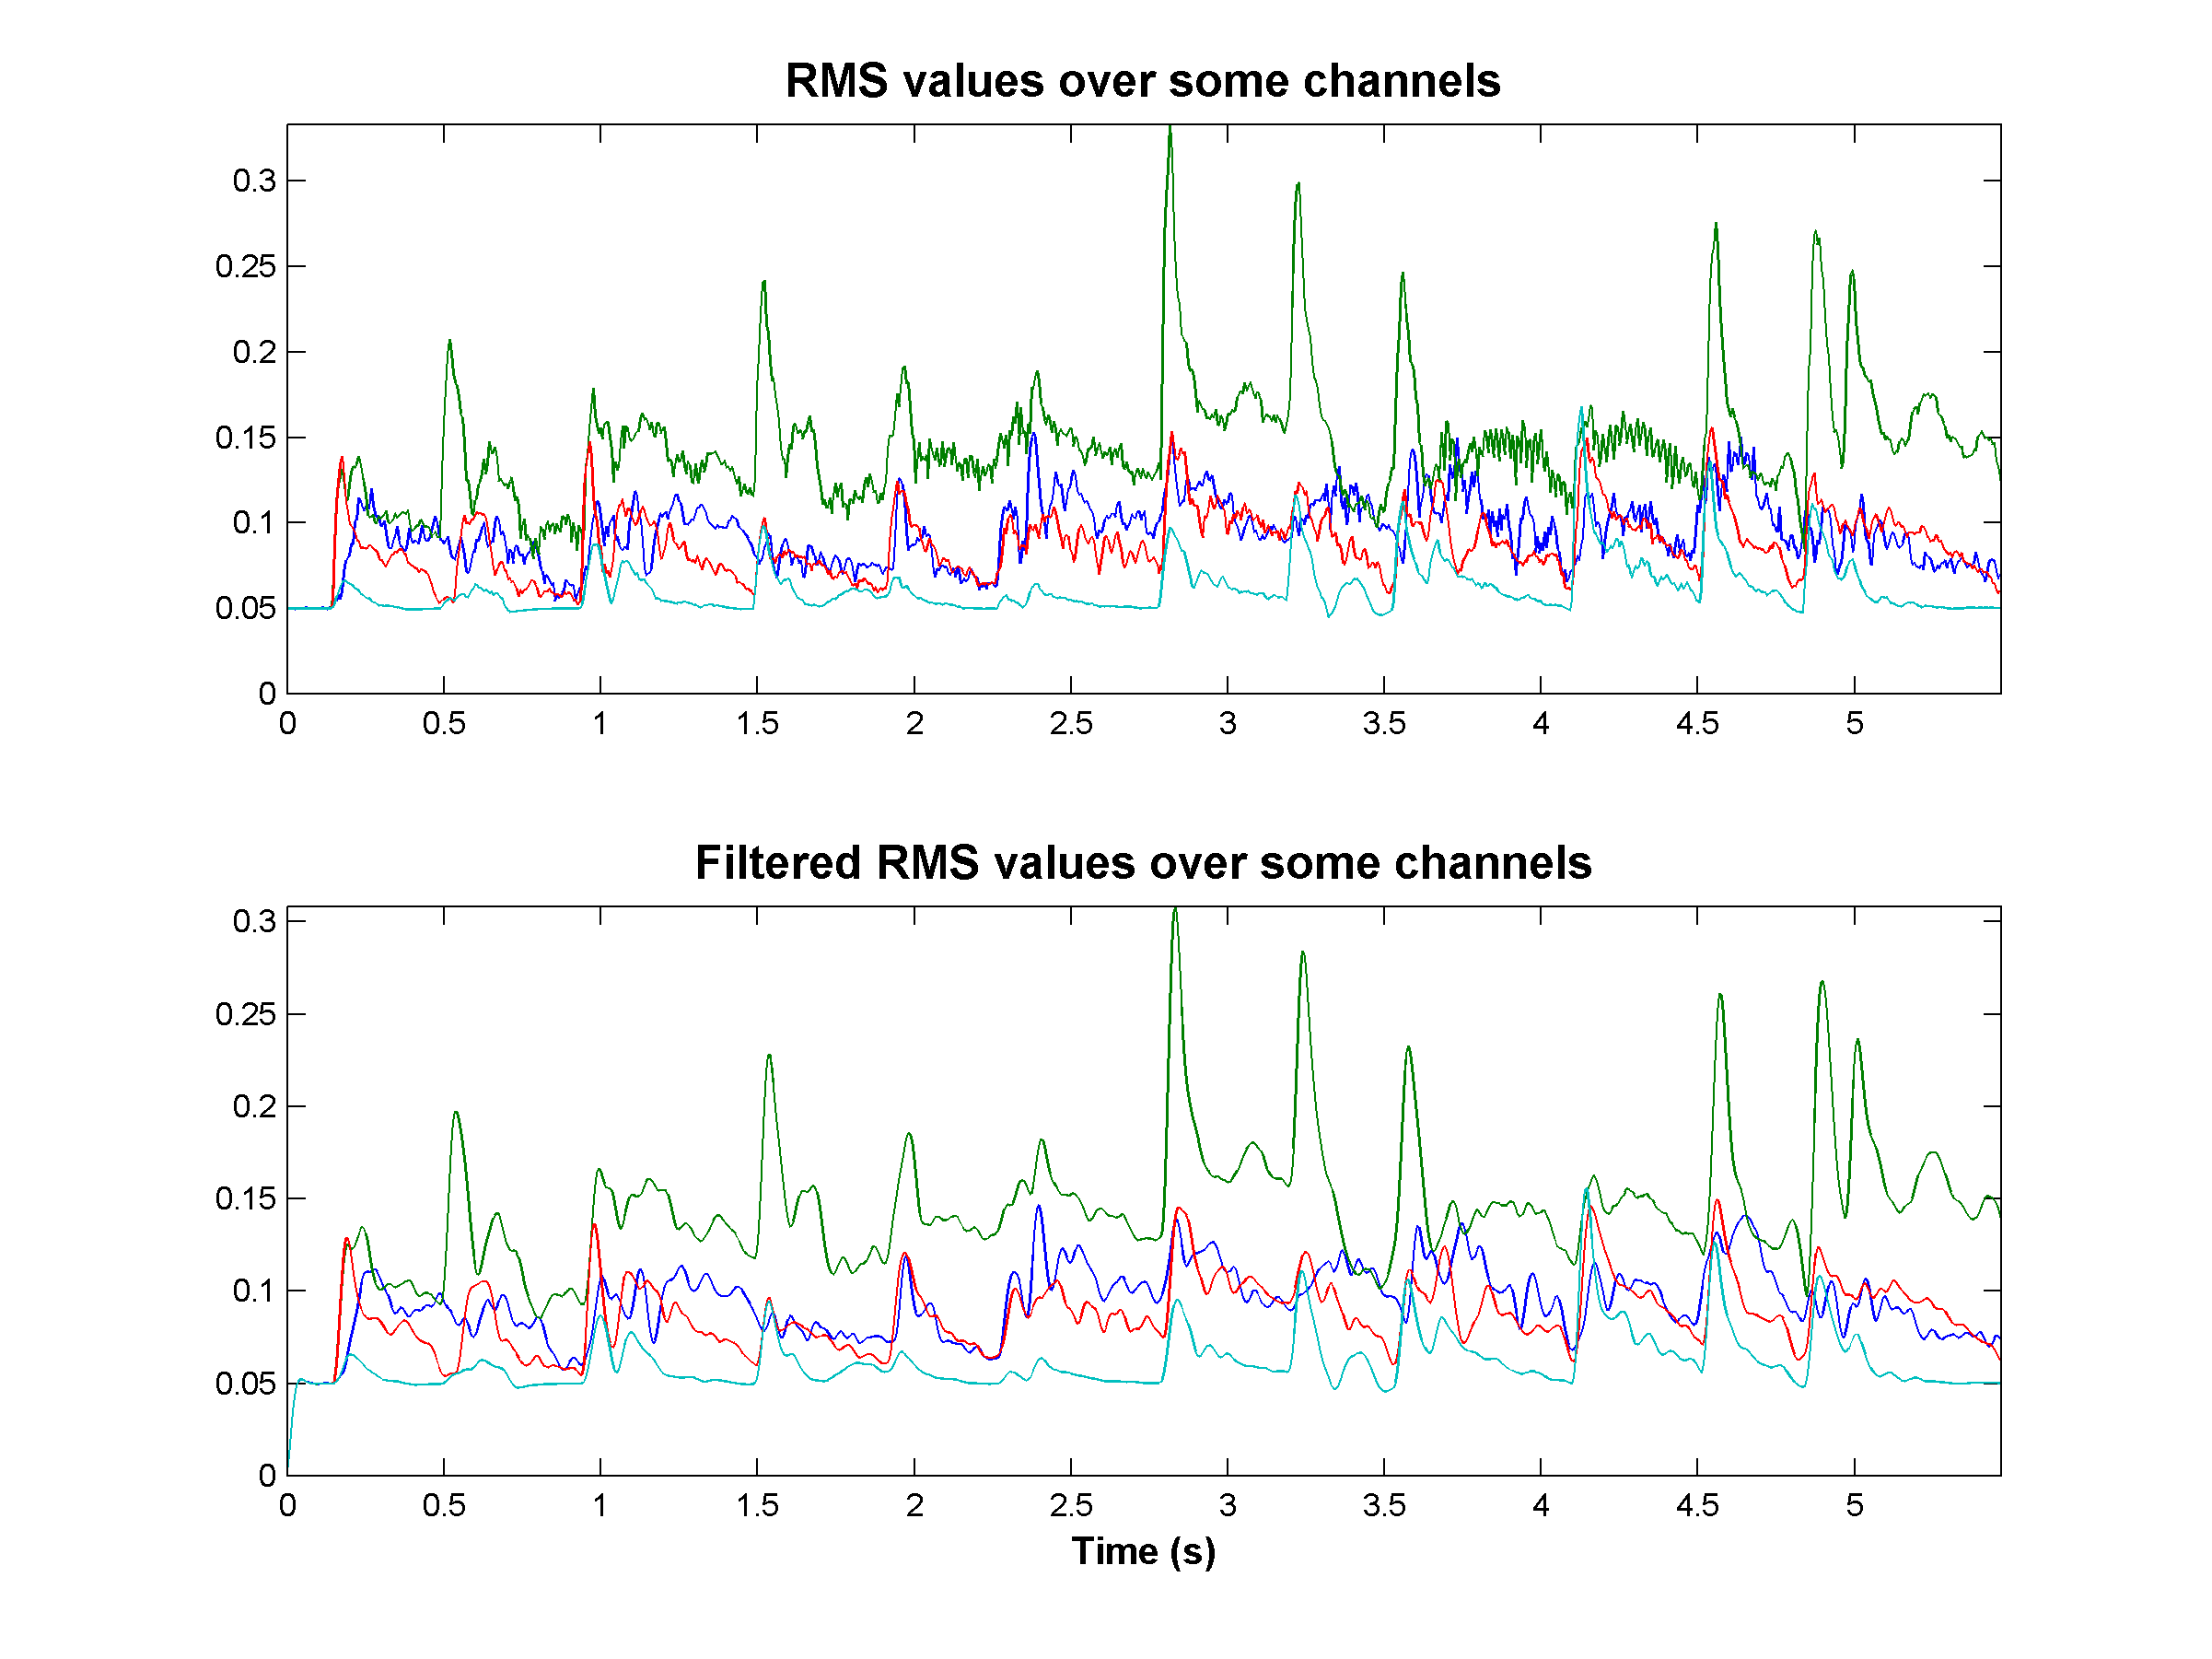
\includegraphics[width=\IPEMDefaultFigureWidth]{Graphics/OnsetsFilteredRMS}
    \caption{Top: RMS values for some channels of the ANI. Bottom: low pass filtered RMS values for the same channels.}
    \label{Fig:OnsetsFilteredRMS}
\end{figure}

\begin{figure}[h]
    \centering
    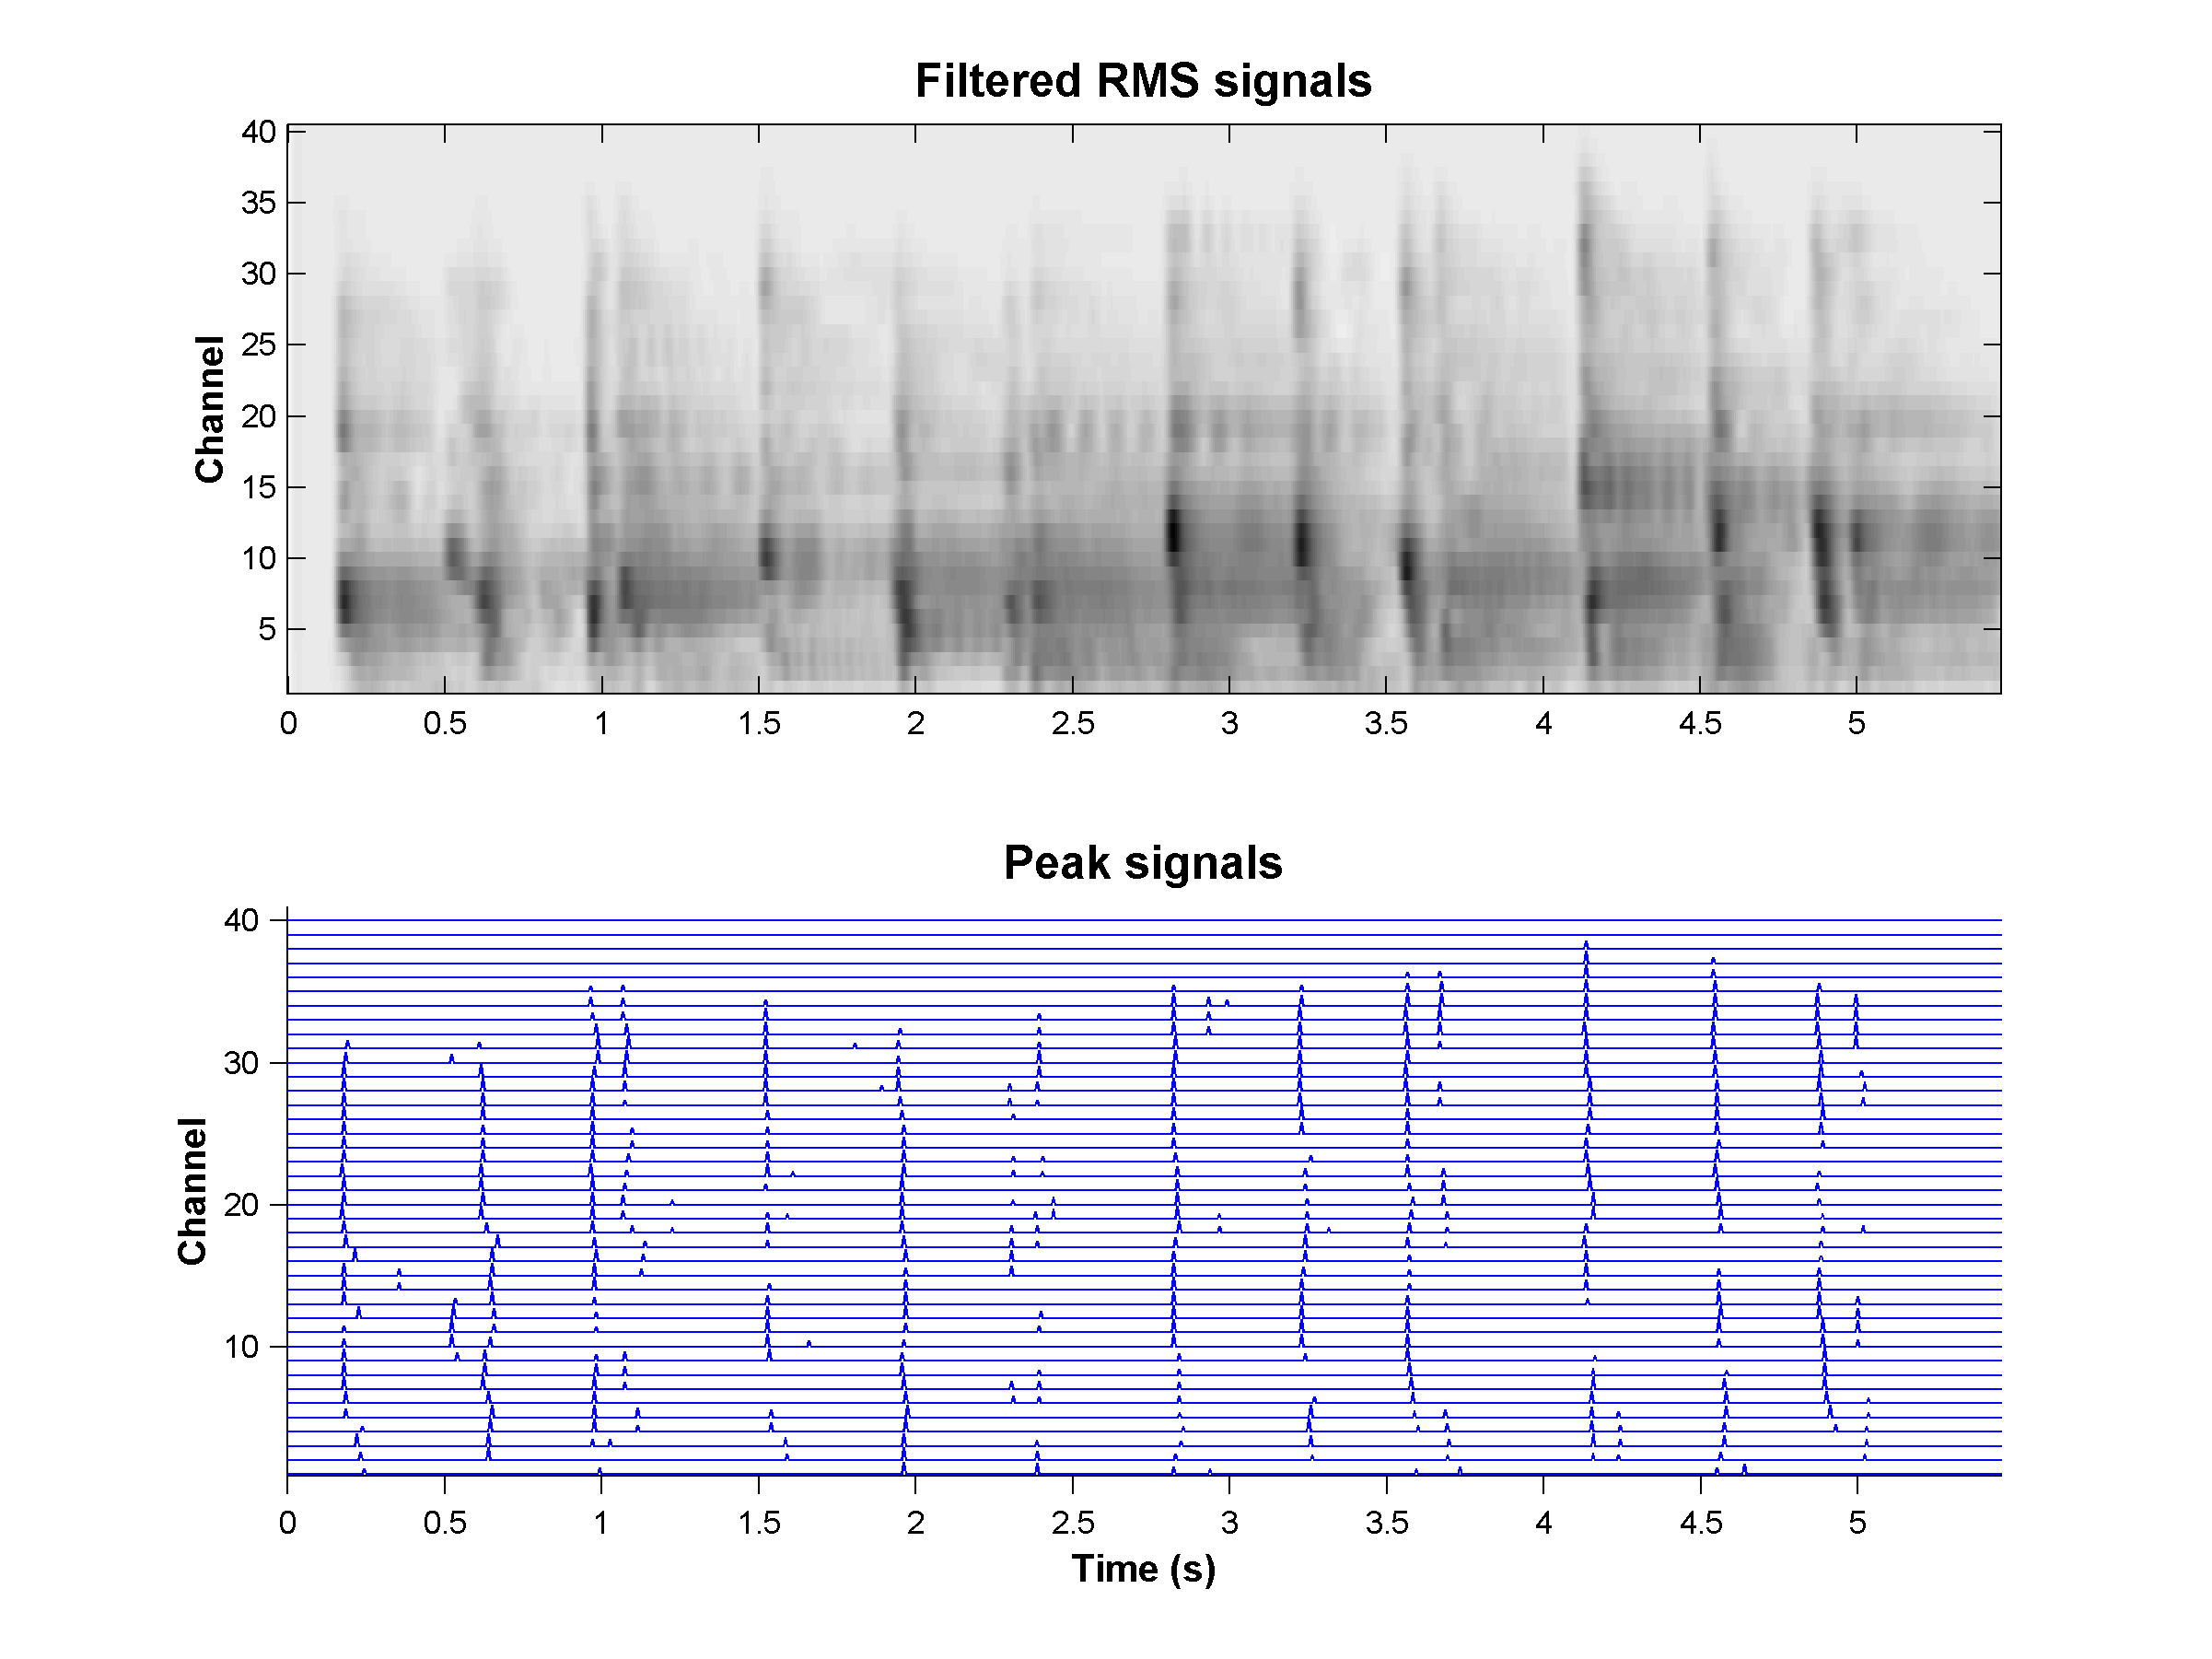
\includegraphics[width=\IPEMDefaultFigureWidth]{Graphics/OnsetsOnsetPeakDetection}
    \caption{Top: filtered RMS values of the ANI. Bottom: peaks detected for each channel.}
    \label{Fig:OnsetsOnsetPeakDetection}
\end{figure}

\begin{figure}[h]
    \centering
    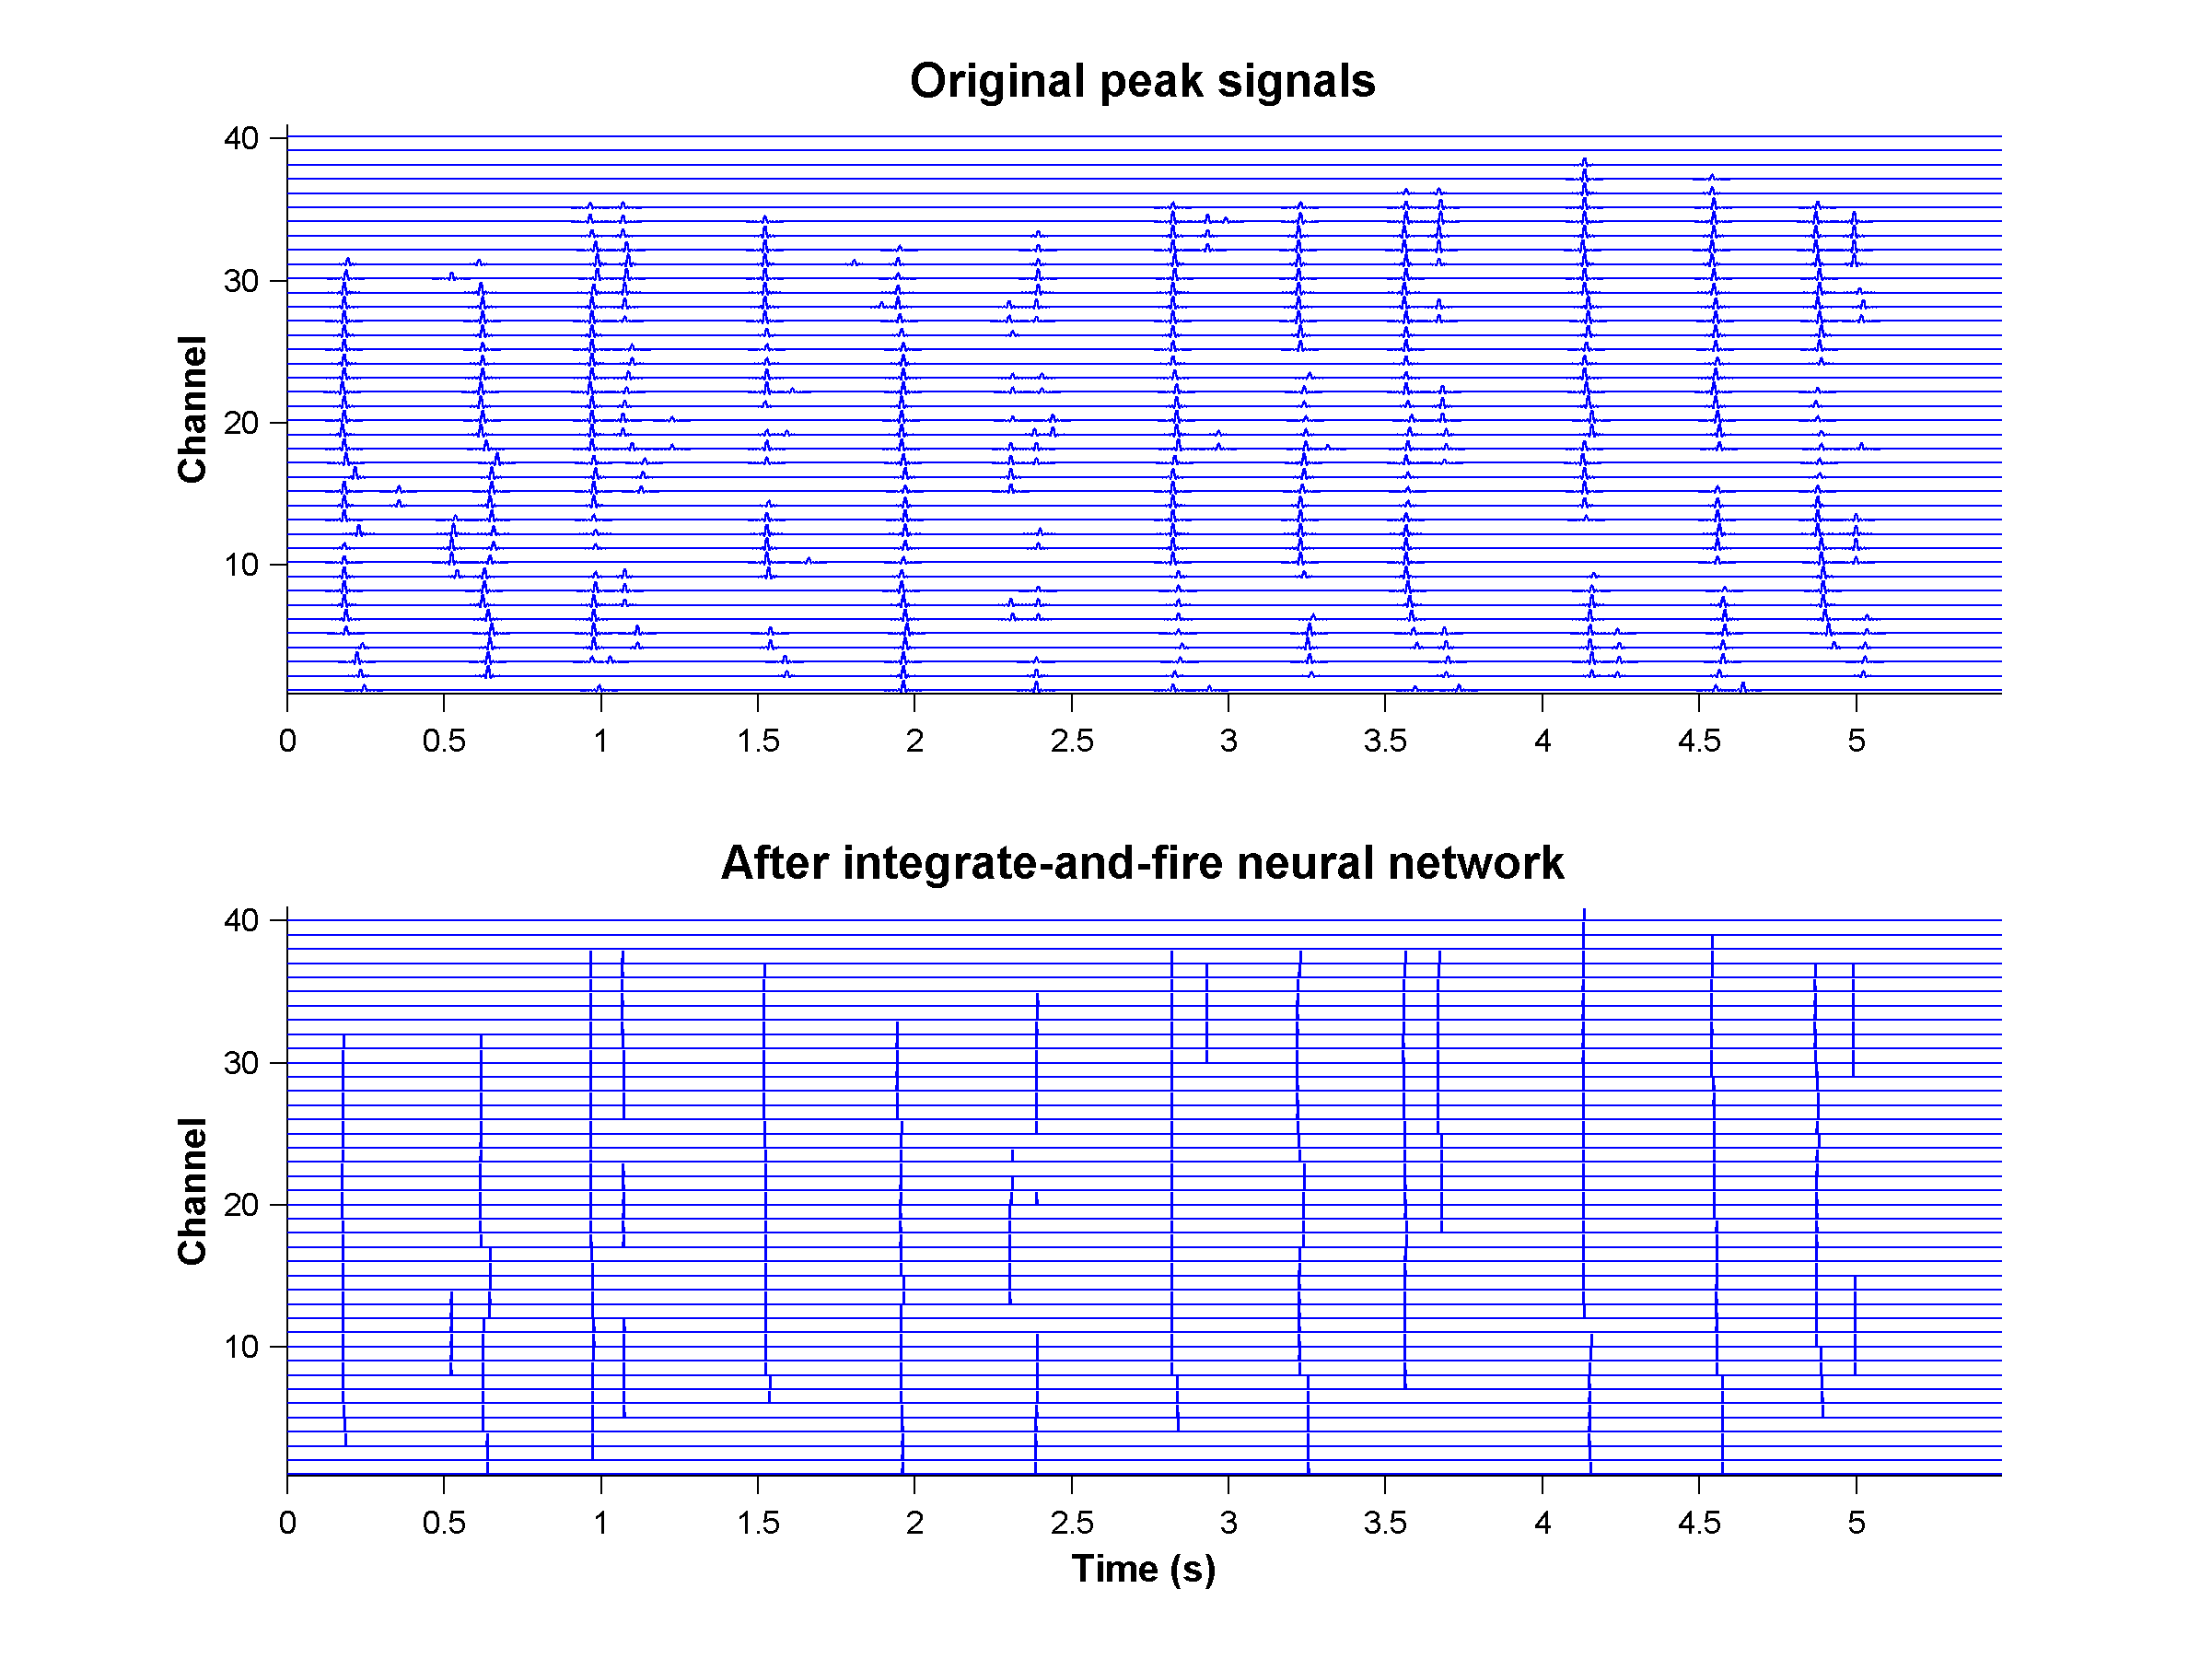
\includegraphics[width=\IPEMDefaultFigureWidth]{Graphics/OnsetsOnsetPattern}
    \caption{Top: detected peaks. Bottom: peaks after applying the integrate-and-fire neural network.}
    \label{Fig:OnsetsOnsetPattern}
\end{figure}

\begin{figure}[h]
    \centering
    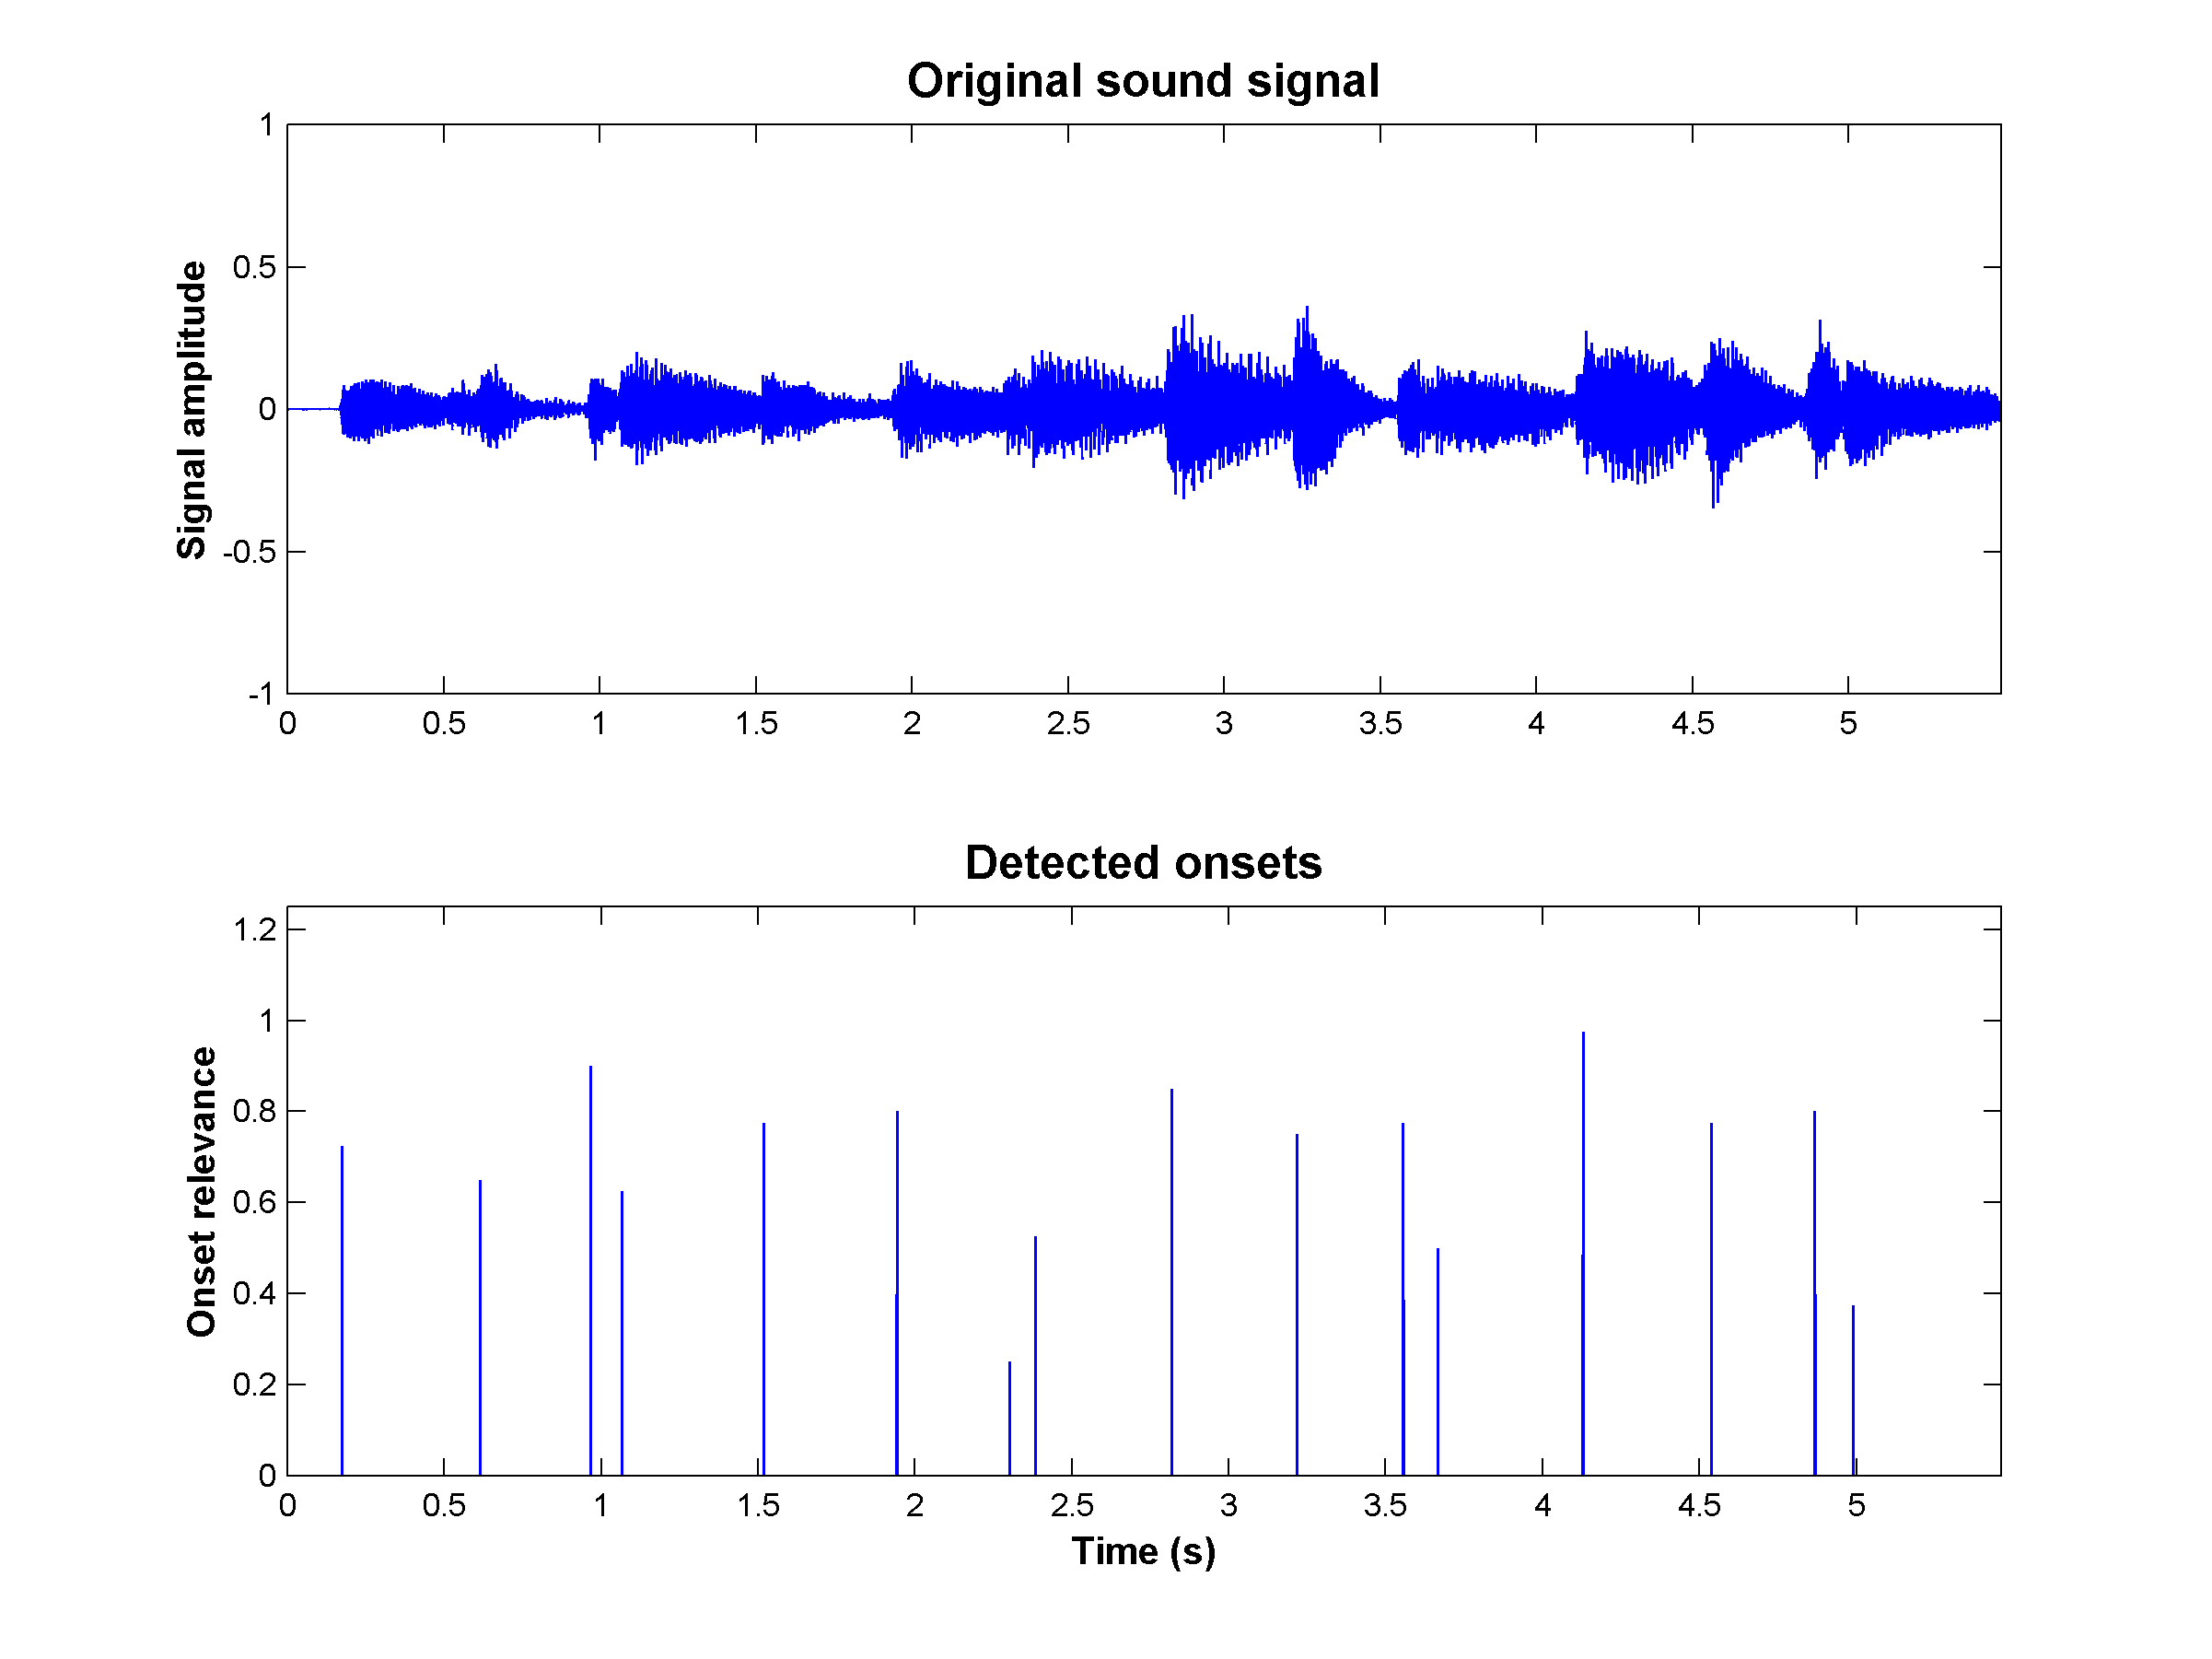
\includegraphics[width=\IPEMDefaultFigureWidth]{Graphics/OnsetsOnsetFilter}
    \caption{Top: original sound signal. Bottom: detected onsets and their relevance level.}
    \label{Fig:OnsetsOnsetFilter}
\end{figure}

\begin{figure}[h]
    \centering
    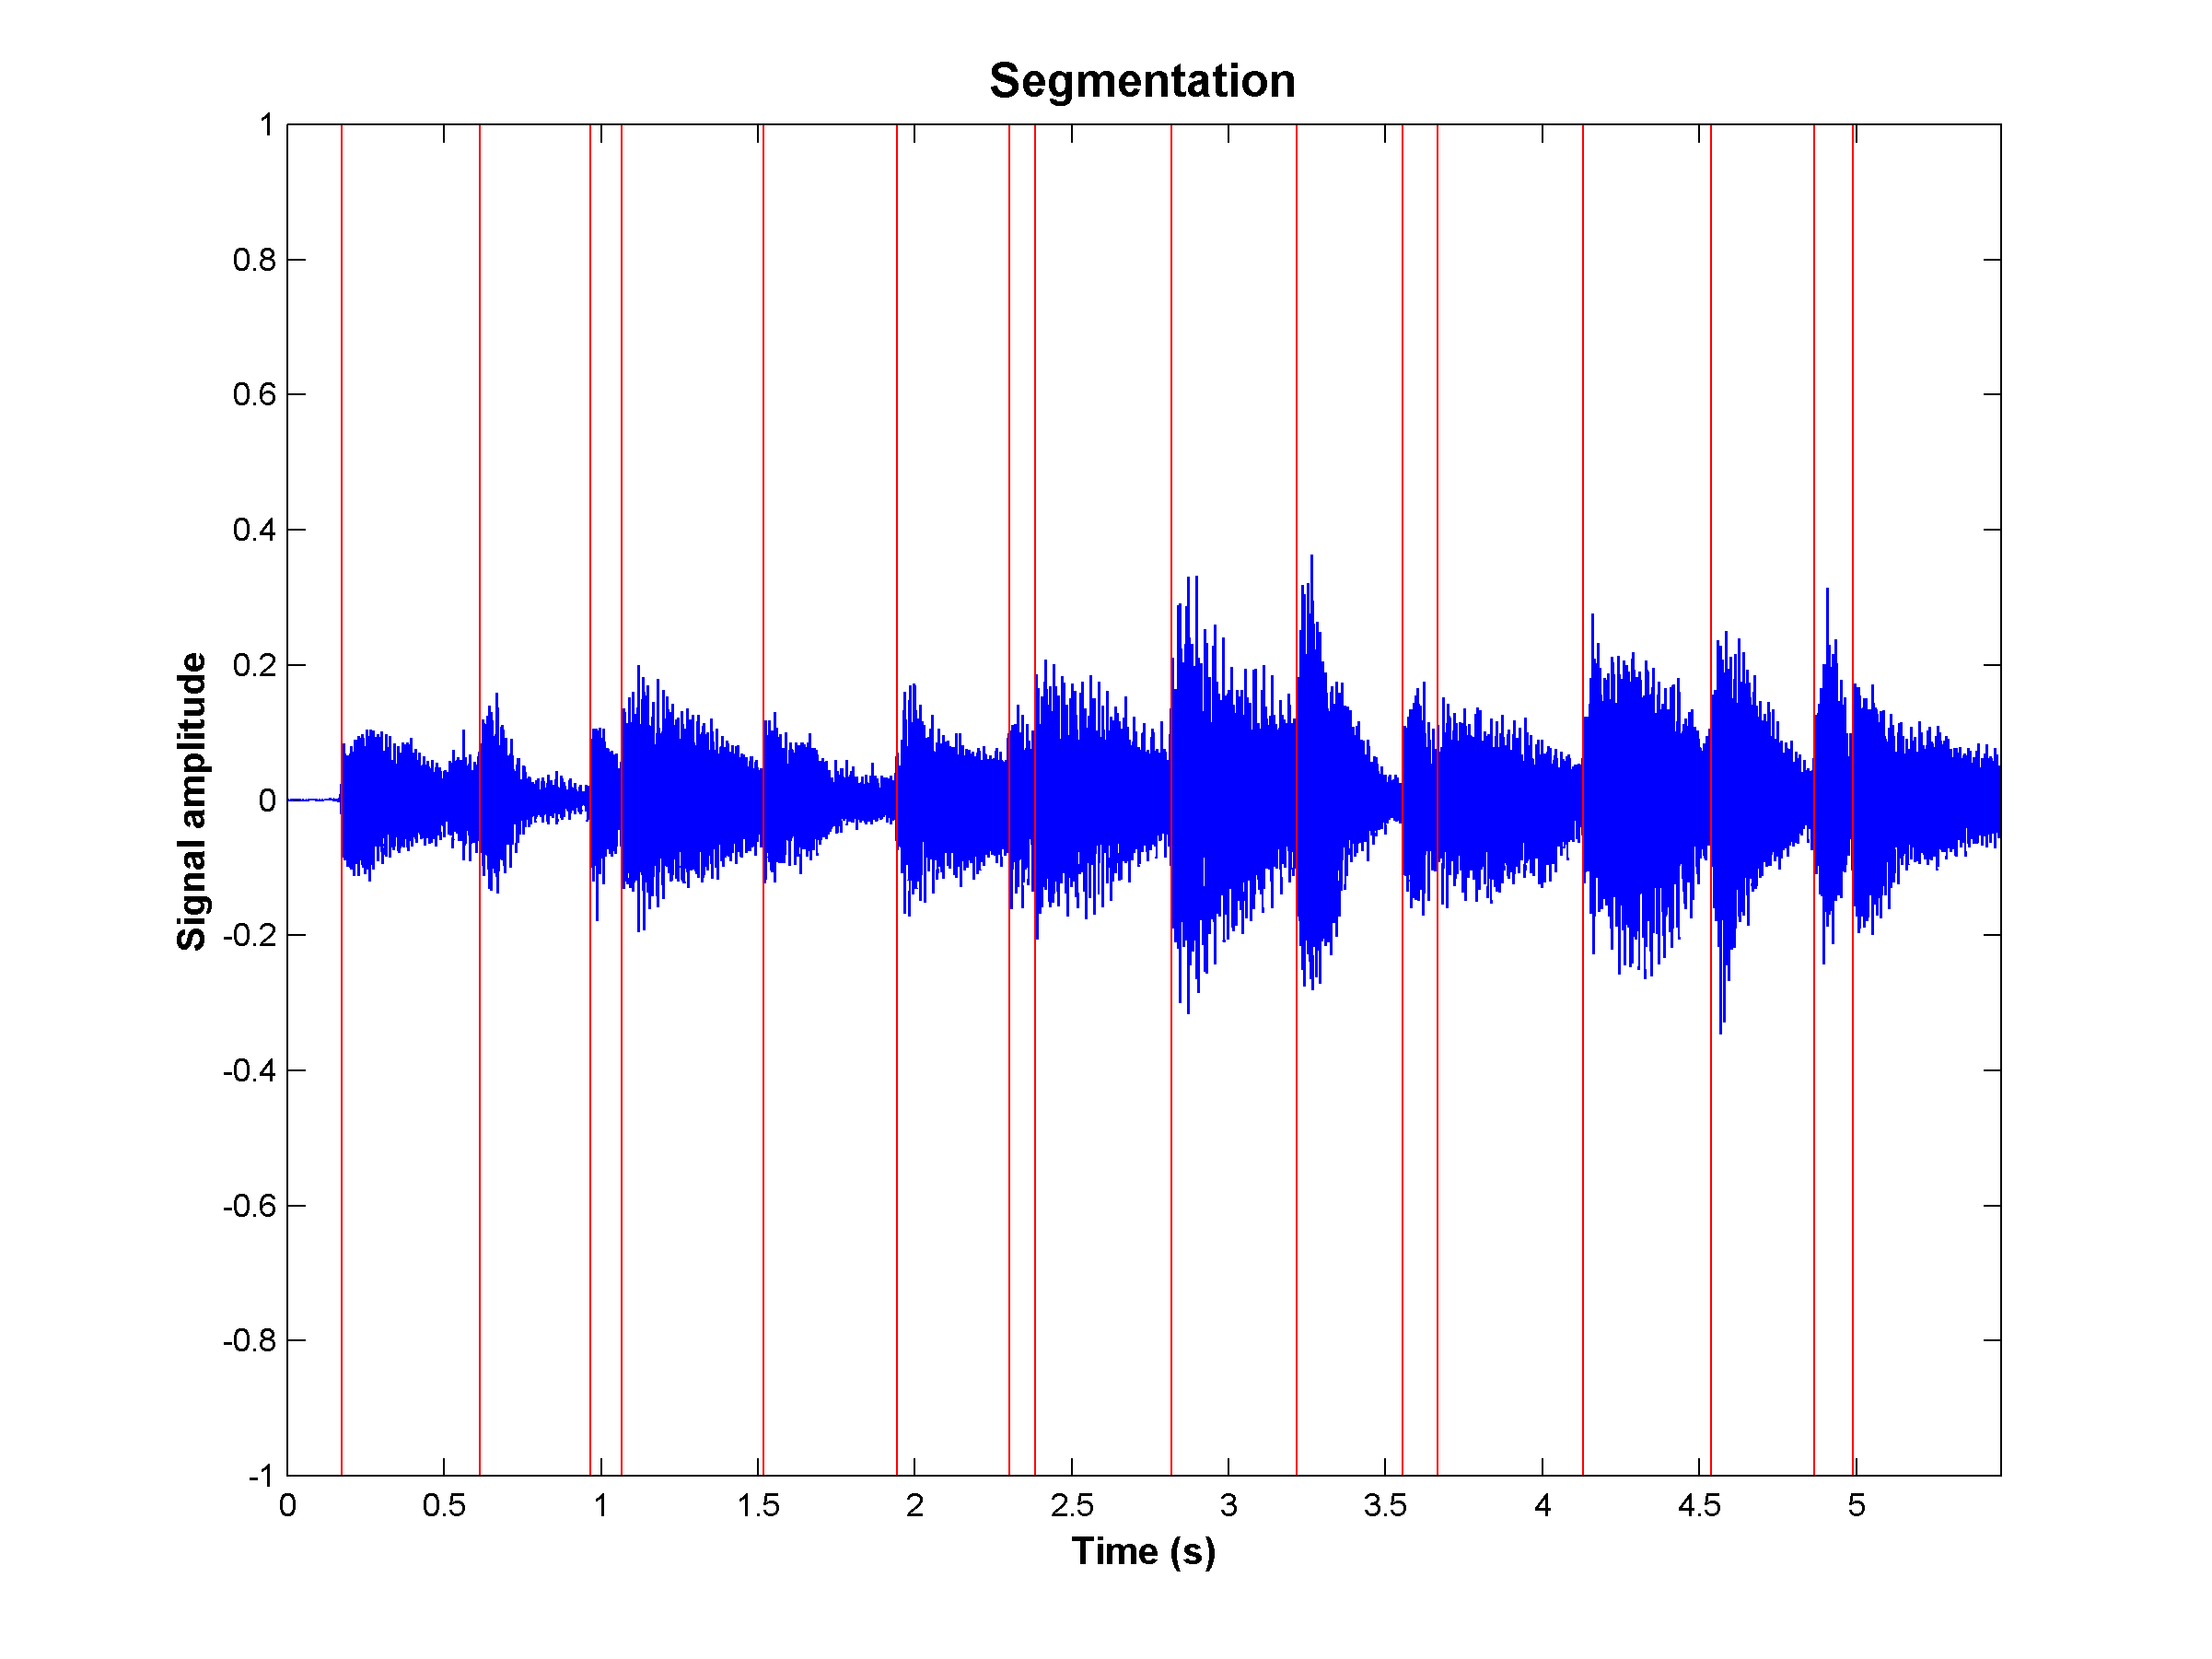
\includegraphics[width=\IPEMDefaultFigureWidth]{Graphics/OnsetsSegmentation}
    \caption{Segmentation of the original sound signal using the onset module.}
    \label{Fig:OnsetsSegmentation}
\end{figure}
